\chapter{Problem Analysis}\label{chapter:analysis}
This chapter analyses the requirements of the project, contrasting the current state of literature to provide a clear list of project objectives and build success criteria for reference on conclusion of the project.

\section{Requirements}
In addition to the research requirements defined for this project, there are also system functionality requirements imposed through expectations of NAC solutions available in industry. Without these additional requirements the system would not be a viable NAC solution.

\subsection{Industry Requirements}
\begin{itemize}
    \item Supporting a large number of EAP-methods, including EAP-TLS, PEAP, EAP-TTLS and EAP-MD5
    \item Allow authentication credentials to be stored centrally in an LDAP server
    \item Allow client access restrictions to be stored in LDAP
    \item Allow IoT devices and other devices incapable of EAP authentication to connect securely to a network
    \item Deny access to the network when a client is not authenticated
    \item Allow both controlled and open ports on the same switch
    \item Be light-weight, not hindering normal functionality of the network
    \item Use exclusively open standards to avoid vendor lock-in
\end{itemize}

\section{Solution Design}
For this project, I propose to provide an 802.1x Authenticator for the Faucet SDN Controller to provide network access control to a Faucet-driven network. 

\subsection{Architecture}
The 802.1x Authenticator application will communicate with the Faucet SDN Controller through the plugin API and must receive EAP requests directly from the network, without them traversing the Faucet Controller.

This can be achieved by exposing the Authenticator to the data network, providing 802.1x as a virtualised network function (VNF).
The port connecting the VNF to the data network is known as a network function virtualisation (NFV) port. Deployment of NFV ports have a number of benefits over using packet-in messages including better scalability independent of the Controller. This approach also removes the ability for unauthenticated users to send traffic directly to the Controller.

All EAPoL traffic from controlled ports must be directed to the closest NFV port using dedicated flow-rules while dropping all other traffic from these ports. Creating these flow-rules will require Faucet to know of NFV ports on startup to ensure traffic is successfully dropped from the required ports. [Refer to Figure \ref{fig:chewie_setup_diagram}]

On successful completion of an authentication attempt, the Authenticator must notify the Controller with the switch, port number and MAC address of the successfully authenticated client. The Authenticator may also provide a VLAN number and/or restriction policies to be applied on the session, if provided by the RADIUS server. The Controller must produce flow-rules in accordance with these requirements and deploy them to the relevant switches.

\begin{figure}\begin{center}
    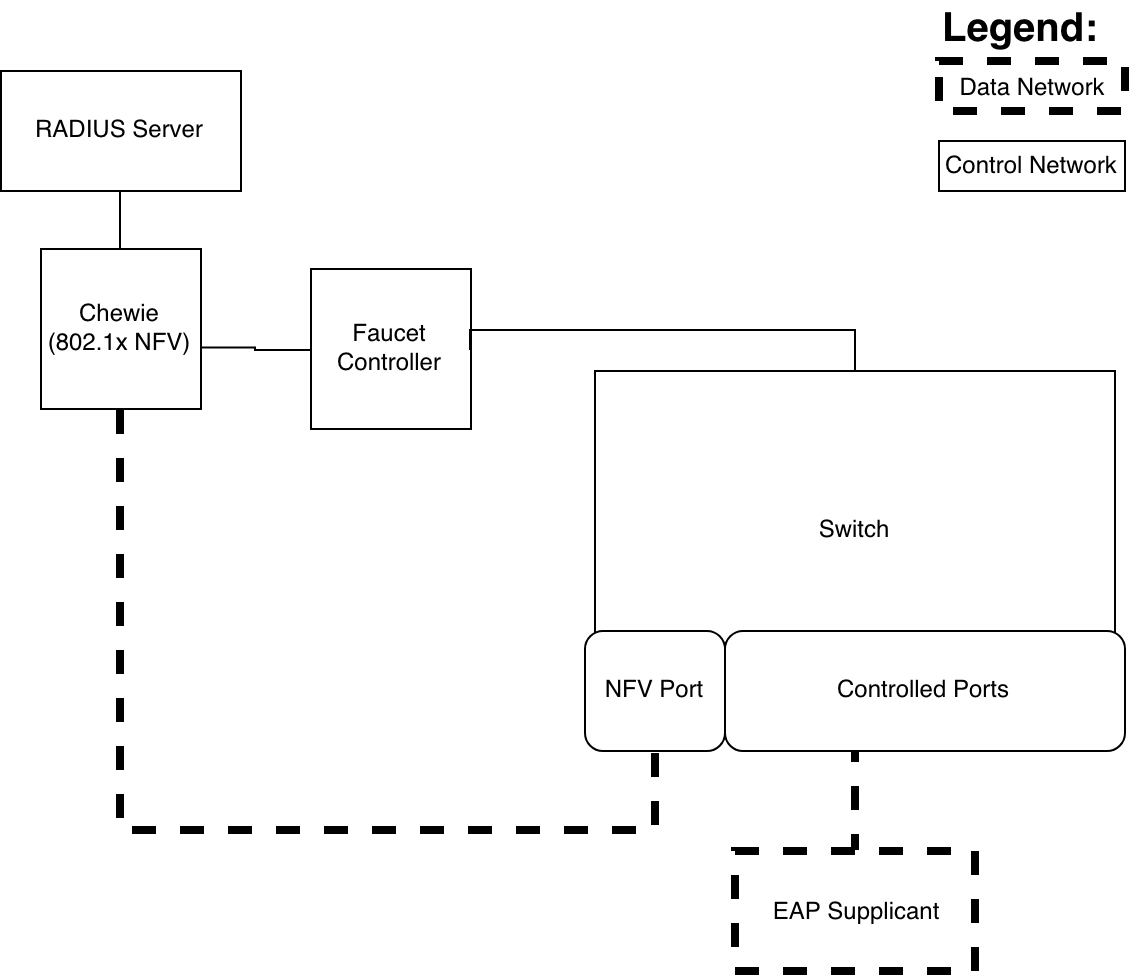
\includegraphics[height=6cm]{images/chewie_architecture.png}
    \caption{Chewie Setup Diagram}
    \label{fig:chewie_setup_diagram}
\end{center}\end{figure}
% no proofread
\subsection{The Authentication Process}
On a switch receiving an authentication request, the frame must be marked with a unique switch and port identification number before it is forwarded to the closest NFV port. This allows the Authenticator to know the origin port of the authentication request.

The Authenticator will perform packet-translation when it receives EAPoL frames. The Ethernet layer must be removed from the EAPoL request exposing the EAP message, which must populate the contents of a RADIUS request before it is forwarded to the RADIUS server. This process is performed in reverse for messages originating from the RADIUS server.

By forwarding EAP requests to the RADIUS server, the Authenticator is not required to perform authentication locally and is implicitly able to perform all EAP-methods supported by the RADIUS server. This allows the Authenticator to remain light-weight while providing all required functionality of a typical NAC system.

The ability to store all credential data in an LDAP service can also be leveraged from the RADIUS server as most common RADIUS servers, such as FreeRadius\cite{freeradius_modules}, provide integration with LDAP services.

Performing EAP authentication on the RADIUS server requires the Authenticator maintain state of the RADIUS communication as it RADIUS challenge-responses require knowledge of previous RADIUS message-authenticator used in the communication. However, this overhead is far outweighed by the leveraged functionality provided by the RADIUS server and can be modelled using a state machine.

\subsection{Authentication Without EAP}
A large number of devices, such as printers and IoT devices, are unable to perform 802.1x authentication due to the EAP requirements. Most IoT devices are unable to perform supplicant duties and this hinders their ability to join secure networks.

The Authenticator for this project must provide a connection mechanism by which these devices are able to securely join a network without removing authentication requirements from the connection port.

Due to this requirement, the Authenticator will provide an alternative to EAP known as mac authentication bypass (MAB). 

MAB provides secure authentication on behalf of a connecting client using their MAC address. This is achieved by sniffing MAC addresses from ingress DHCP requests from controlled ports. These MAC addresses can be used by the Authenticator to perform a RADIUS authentication process on behalf of the new client. \cite{junos_mab_switching}

As there is no standardised protocol for MAB leaving the format of the MAC credentials in the RADIUS server ambiguous. To perform successful authentication the format of MAC address in RADIUS must be known by the Authenticator. For this project I will be expecting MAB credentials will consist of MAC addresses stored as both user-name and password, without separating colons. This format may differ depending on the Authenticator and the vendor providing the devices.\cite{junos_mab_setup} \cite{hpe_mab_setup}

On successful authentication, the Authenticator will receive all session restriction policies and VLAN information where applicable. These requirements will be provided to the Controller where the appropriate flows must be built and distributed to the relevant switches.

If the authentication process is not successful, all traffic from the client will be dropped.

As MAB authentication is performed by the Authenticator, the connecting client is not aware the authentication process has occurred. Also, the Authenticator requires the connecting device use DHCP. If a local static IP address is configured on the connecting devices the authentication process will not trigger and the port will remain closed.

MAB is less secure than an EAP-based authentication method as devices can be configured to spoof user-defined MAC addresses, but as there are many devices unable to perform EAP this is a secure alternative to providing an unprotected port for these devices. 

As MAB is less secure that EAP, it will required to be explicitly applied to a controlled port.